\documentclass{article}

\usepackage[hyphens]{url} 


\usepackage[utf8]{inputenc}

\usepackage{pdfpages}
\usepackage{lastpage}
\usepackage{fancyhdr}
\usepackage{ngerman}
\usepackage{listings}
\usepackage{hyperref}
\usepackage{tabularx}
\usepackage{floatrow}
\usepackage[tableposition=top]{caption}
\floatsetup[table]{capposition=top}

\usepackage{amsmath, amssymb}

\usepackage[utf8]{inputenc}

\usepackage{xifthen}
\usepackage[numbib]{tocbibind}

\newcommand\twodigits[1]{%
   \ifnum#1<10 0#1\else #1\fi
}



\lhead{Phase und Leistung}
\rhead{27. November 2020\\T. Maier, J. Winkler}
%\cfoot{\twodigits{\thepage}~/ \pageref{LastPage}}
\cfoot{{\thepage}~/ \pageref{LastPage}}

\newcommand{\W}{\text{W}}
\newcommand{\V}{\text{V}}
\newcommand{\A}{\text{A}}

\newcommand{\UR}{$U_R$ }
\newcommand{\UIR}{$U_\text{IR}$ }

\newcommand{\mini}{\operatorname{min}}



\definecolor{commentgreen}{RGB}{2,112,10}
\definecolor{eminence}{RGB}{108,48,130}
\definecolor{weborange}{RGB}{255,165,0}
\definecolor{frenchplum}{RGB}{129,20,83}

\lstdefinelanguage{python}{
    morekeywords={def, for, range, abs, return},
    otherkeywords={<-,->, |>, \%\{, \}, \{, \, (, )},
    sensitive=true,
    morecomment=[l]{\#},
    morecomment=[n]{/*}{*/},
    morecomment=[s][\color{purple}]{:}{\ },
    morestring=[s][\color{orange}]"",
    commentstyle=\color{commentgreen},
    keywordstyle=\color{eminence},
    stringstyle=\color{red},
	basicstyle=\ttfamily,
	breaklines,
	showstringspaces=false,
	frame=tb
}
\lstset{
extendedchars=\true,
inputencoding=utf8
}




\begin{document}

\parindent0cm

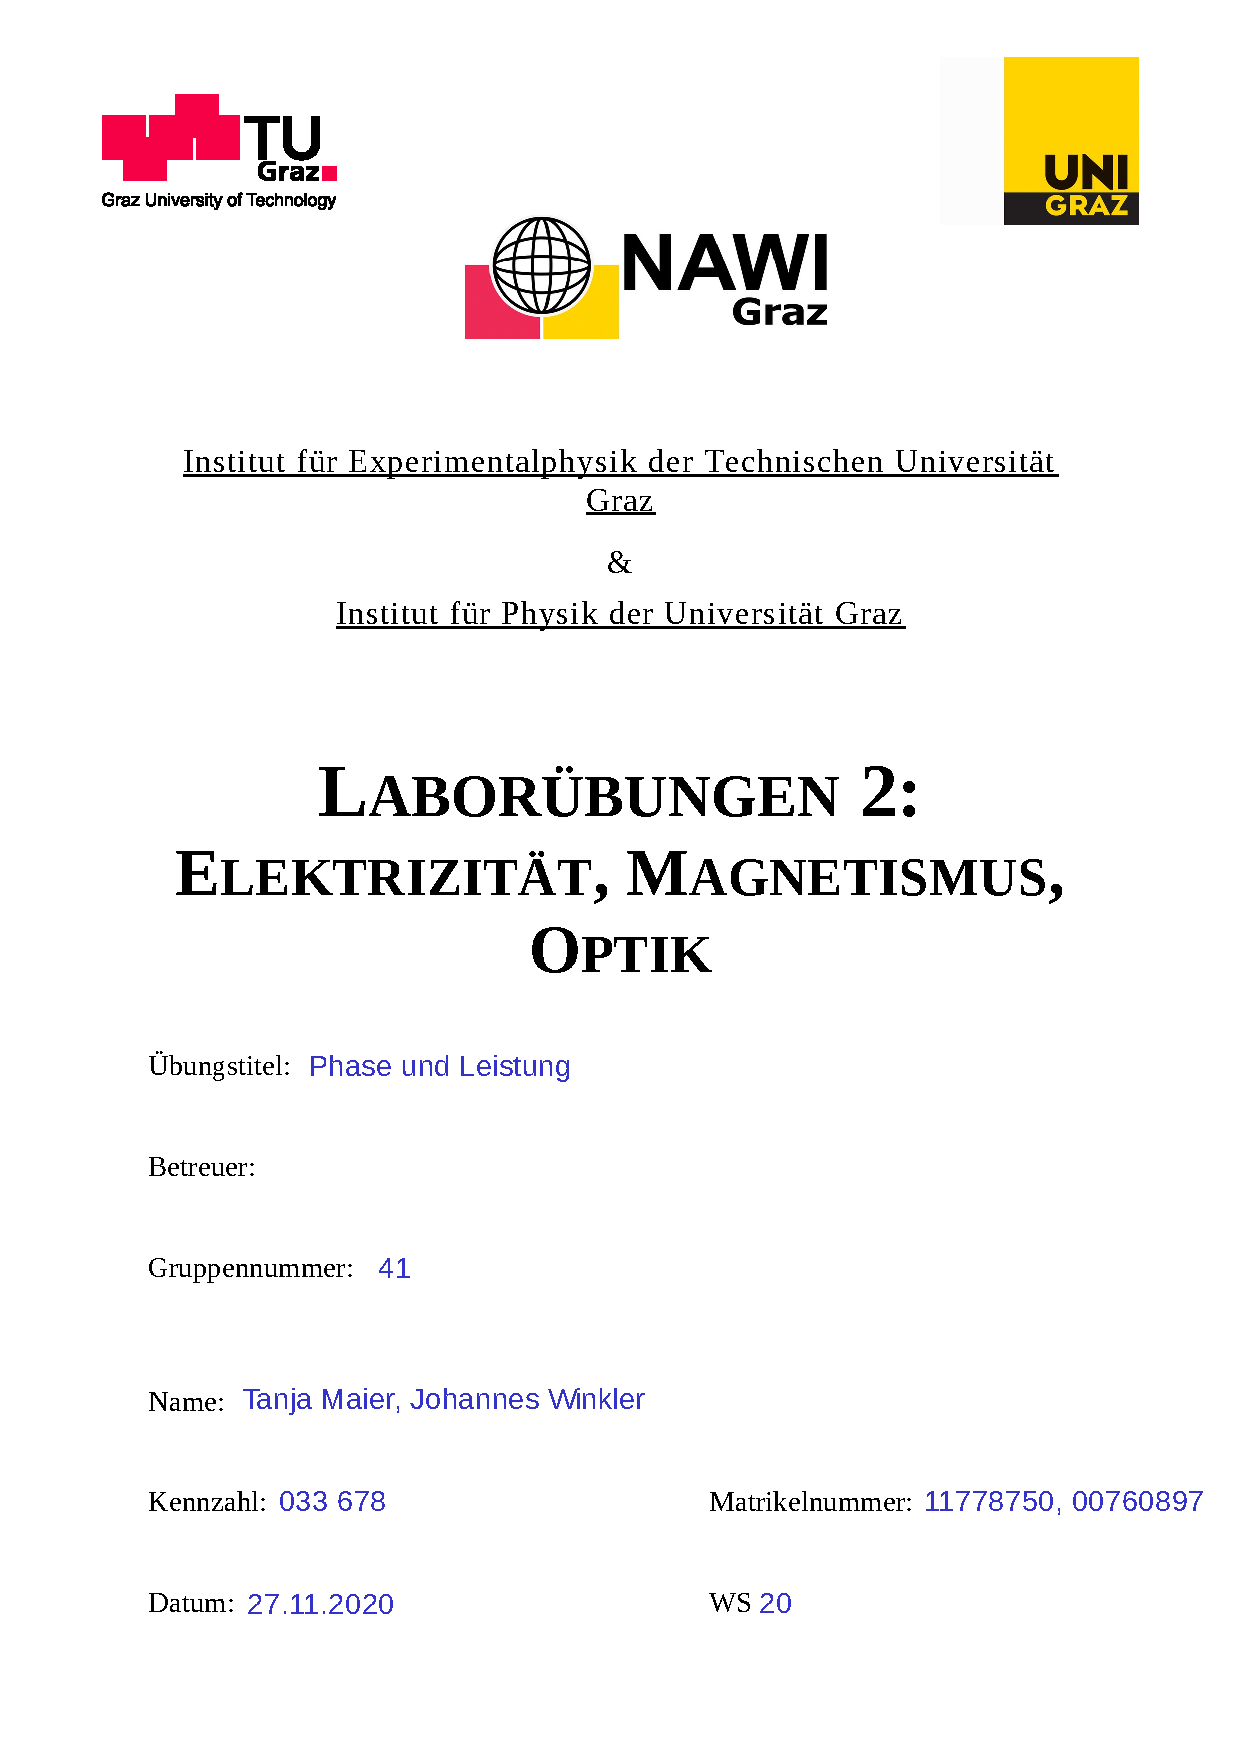
\includepdf{Deckblatt.pdf}


\pagestyle{fancy}

\tableofcontents
\newpage
\section{Aufgabenstellung}

\begin{enumerate}
\item Untersuchung  der  Anzeige  von  unterschiedlichen  Spannungsmessinstrumenten  bei verschiedenen Kurvenformen.
\item Messtechnische Ermittlung der Phasenlage von Strom und Spannung an einem Kondensator.
\item Messtechnische Ermittlung der Phasenlage von Strom und Spannung an einer Spule.
\item Messtechnische Ermittlung der elektrischen Leistung in einer RC-Schaltung.
\item Messtechnische Ermittlung der elektrischen Leistung in einer RL-Schaltung.
\end{enumerate}

\section{Voraussetzungen und Grundlagen}

\subsection{Wechselstrom und Wechselspannung}

Als Wechselstrom bezeichnet man jene Art von elektrischem Strom, bei der sich die Stärke und die Richtung periodisch ändern. Damit einhergehend ändert sich auch die Spannung und wird daher als Wechselspannung bezeichnet. Wichtige Größen sind hier der Scheitelwert (Maximalbetrag des Augenblickwertes bei einem Wechselsignal) und die sogenannten Effektivwerte $I_\text{eff}$ und $U_\text{eff}$. Dies sind jene Werte, bei denen im Wechselstromkreis die gleiche Leistungsabgabe, wie beim Gleichstromkreis (also keine periodische Änderung von Stärke und Richtung des Stroms) mit denselben Werten erfolgt.
\begin{align}
U_\text{eff} &= \sqrt{ \frac{1}{\tau}\cdot \int_0^\tau u^2(t)\cdot dt } \\ I_\text{eff} &= \sqrt{ \frac{1}{\tau}\cdot \int_0^\tau i^2(t)\cdot dt }
\end{align}
dabei ist $u(t)$ der Augenblickswert der Spannung, $i(t)$ der Augenblickswert des Stroms und $\tau$ die Periodendauer des Signals.
Zudem kann aus diesen Größen auch der Scheitelfaktor berechnet werden, der das Verhältnis von Scheitelwert zu Effektivwert (sowohl für Strom als auch für Spannung) darstellt.
\begin{align}
f_s &= \frac{U_s}{U_\text{eff}} \\
f_s &= \frac{I_s}{I_\text{eff}} 
\end{align}
Ähnlich zum Effektivwert lässt sich auch der Gleichrichtwert für Strom und Spannung als zeitliches Mittel berechnen
\begin{align}
U_\text{gl} &= \frac{1}{\tau}\cdot \int_0^\tau \left|u(t)\right|\cdot dt  \\ I_\text{gl} &= \frac{1}{\tau}\cdot \int_0^\tau \left|i(t)\right|\cdot dt 
\end{align}
Der Formfaktor (Verhältnis von Effektivwert zu Gleichrichtwert) ergibt sich dann als
\begin{align}
f_f &= \frac{U_\text{eff}}{U_\text{gl}} \\
f_f &= \frac{I_\text{eff}}{I_\text{gl}} 
\end{align}
Wichtig zu beachten ist, dass Scheitelfaktor und Formfaktor vom zeitlichen Verlauf des Signals abhängen dementsprechend unterschiedliche Werte liefern. (vgl. \cite{moodle}, \cite{src2}, \cite{src3}, \cite{src4}, \cite{src5})


\subsection{Messung von Gleichrichtwert und Effektivwert}

Um schnelle Änderungen erfassen zu können zeigen Messgeräte meist gemittelte Werte an (elektronisch gemittelt z.B. mit dem Dual-Slope-Verfahren). Diese Erfassung der Wechselgröße erfolgt meist über die Messung der Gleichrichtwertes, da dies im Gegensatz zur Messung des Effektivwertes weniger aufwändig ist.



\subsection{Wechselstromwiderstände und deren Leistung}

Hierbei wird unterschieden zwischen Wirkleistung, Blindleistung und Scheinleistung. Die Wirkleistung ist jener Teil der Leistung, der in mechanische Arbeit umgewandelt wird. In einem Wechselstromkreis erfolgt hier eine Umwandlung von elektrischer in thermische Energie. Die Wirkleistung kann durch
\begin{align}
P = U\cdot I \cdot \cos(\phi)
\end{align}
beschrieben werden, wobei $U$ die Spannung und $I$ der Strom ist. $\phi$ ist die Phasenverschiebung. Man erkennt relativ leicht, dass die Leistung maximal wird, wenn die Phasenverschiebung gleich 0 ist ($\cos(0)=1$). (vgl. \cite{moodle}, \cite{src6})


Die Blindleistung wird zum Aufbau bzw. zum Abbau von elektromagnetischen Feldern benötigt und ergibt sich aus
\begin{align}
Q = U\cdot I \cdot \sin	(\phi)
\end{align}
wobei diese bei einer Phasenverschiebung von $\dfrac{\pi}{2}$ maximal wird.(vgl. \cite{moodle}, \cite{src6})


Die Scheinleistung ist die Gesamtleistung, die sich aus Wirkleistung und Blindleistung ergibt. Sie ergibt sich durch vektorielle Addition von $P$ und $S$
\begin{align}
S = P^2 + Q^2 = U\cdot I 
\end{align}


\subsection{Impedanzen}




\section{Geräteliste}

\begin{table}[H]
\caption{Liste der verwendeten Geräte}

~

\begin{tabular}{l|p{2.5cm}p{3cm}lll}
Abk. & Gerätename    &  Modell/Wert  & Unsicherheit\\
\hline
N & Netzgerät & Hameg HM8040-2 \\
FG & Funktions\-generator & Hameg HM8030-3 \\
OS & Oszilloskop & DSO-X 2002A \\
R & Widerstand & $R=68.0~\Omega$ & $\Delta R = 3.4~\Omega$ \\
C1 & Kondensator & $C_1=100~\mu$F & $\Delta C_1 = 20~\mu$F \\
C2 & Kondensator & $C_2=47~\mu$F & $\Delta C_2 = 10~\mu$F \\
C3 & Kondensator & $C_3=20~\mu$F & $\Delta C_3 = 4~\mu$F \\
C4 & Kondensator & $C_3=10~\mu$F & $\Delta C_3 = 2~\mu$F \\
\end{tabular}
\end{table}

Sämtliche Daten wurden nach den Versuch mit Python3.8 ausgewertet, wobei für Grafiken die Library \texttt{Matplotlib} verwendet wird. 





\section{Beschreibung der Versuchsanordnung}


\subsection{Untersuchung  der  Anzeige  von  unterschiedlichen  Spannungsmessinstrumenten  bei verschiedenen Kurvenformen}
\label{subsec:aufbau_task1}

Der Hameg HM8030-3 Funktionsgenerator wird verwendet um verschiedene Spannungskurven zu erzeugen. Dann wird die Spannung einmal mit dem Oszilloskop gemessen (inkl. Spitze-Spitze-Wert und Effektivwert). Zusätzlich noch mit 3 weiteren Messgeräten: TTi1604, M4600 und Unigor 4.


\begin{figure}[H]
\centering
\caption{Versuchsaufbau, Aufgabe 1}
\label{fig:aufbau_task1}
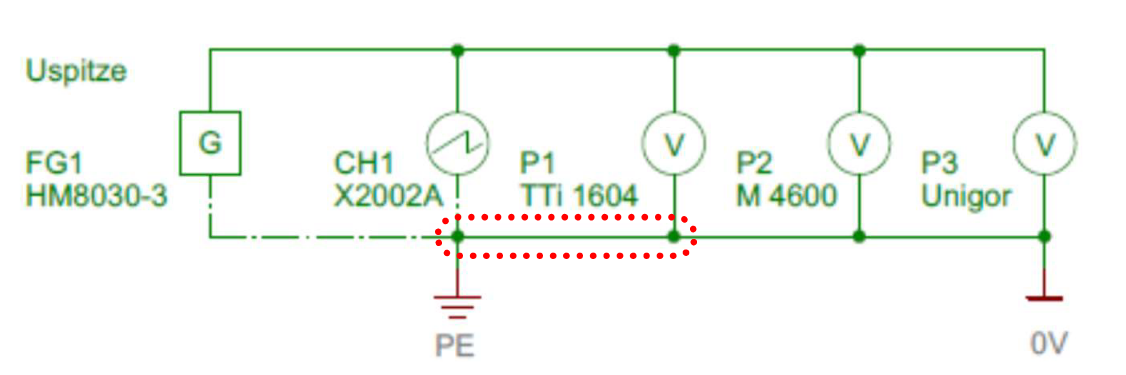
\includegraphics[scale=1]{bilder/aufbau_task1.png}
\end{figure}


\subsection{Phasenlage von Strom und Spannung an einem Kondensator bzw. einer Spule}

In diesem Versuch wird zweimal derselbe Versuchsaufbau verwendet, wobei der Kondensator für den dritten Versuch durch eine Spule ersetzt wird. Die Aufbauten sind in Grafiken~\ref{fig:aufbau_task2} und \ref{fig:aufbau_task3} zu sehen. CH2 misst die betreffende Spannung an Kondensator bzw. Spule, während CH1 für die Berechnung des dazugehörigen Stromes herangezogen wird.

Für das Signal wird in beiden Fällen ein Transformator herangezogen. Als Bezugspunkt für die Messung der Spannung wird in beiden Fällen das Verbindungsstück zwischen dem Widerstand und dem zu vermessenden Bauteil definiert.

\begin{figure}[H]
\centering
\caption{Versuchsaufbau, Aufgabe 2}
\label{fig:aufbau_task2}
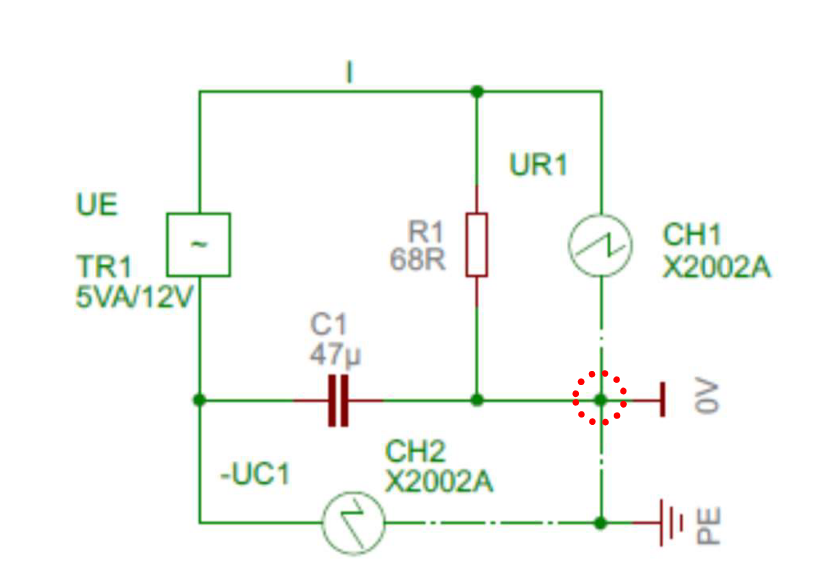
\includegraphics[scale=1]{bilder/aufbau_task2.png}
\end{figure}



\begin{figure}[H]
\centering
\caption{Versuchsaufbau, Aufgabe 3}
\label{fig:aufbau_task3}
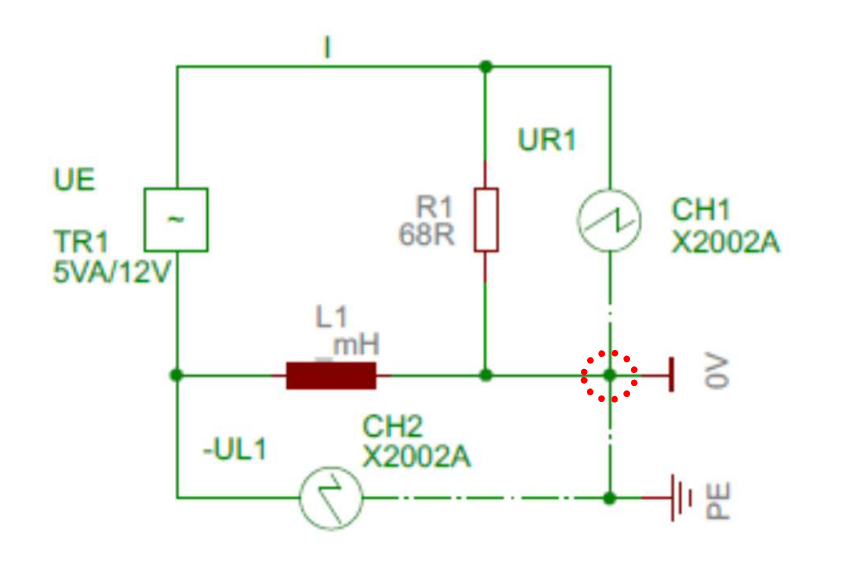
\includegraphics[scale=1]{bilder/aufbau_task3.png}
\end{figure}


\subsection{Leistung einer RC- bzw RL-Schaltung}

\begin{figure}[H]
\centering
\caption{Versuchsaufbau, Aufgabe 4}
\label{fig:aufbau_task4}
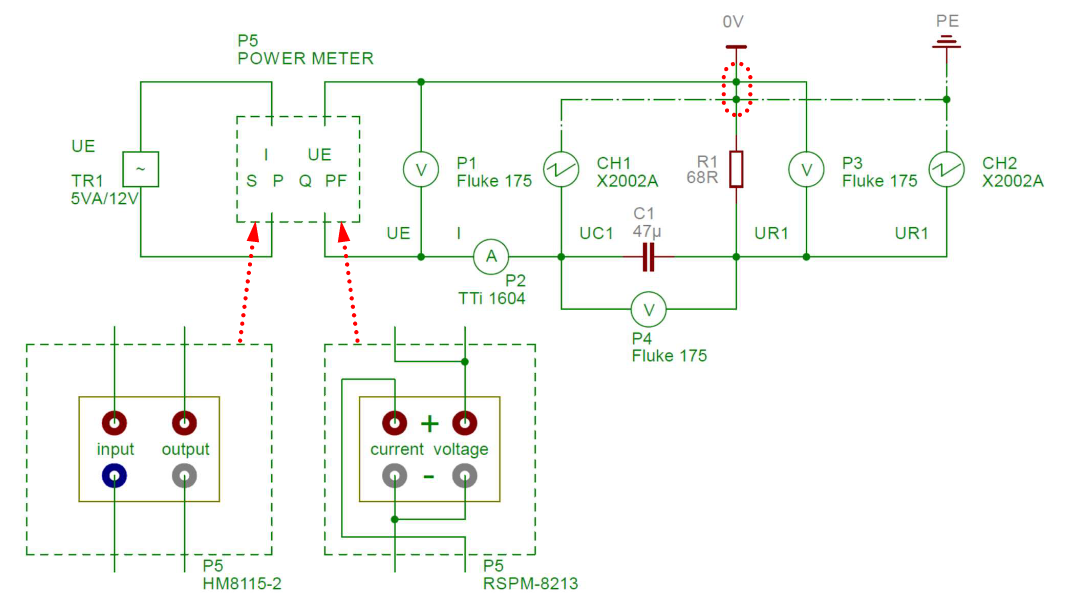
\includegraphics[scale=1]{bilder/aufbau_task4.png}
\end{figure}



\begin{figure}[H]
\centering
\caption{Versuchsaufbau, Aufgabe 5}
\label{fig:aufbau_task5}
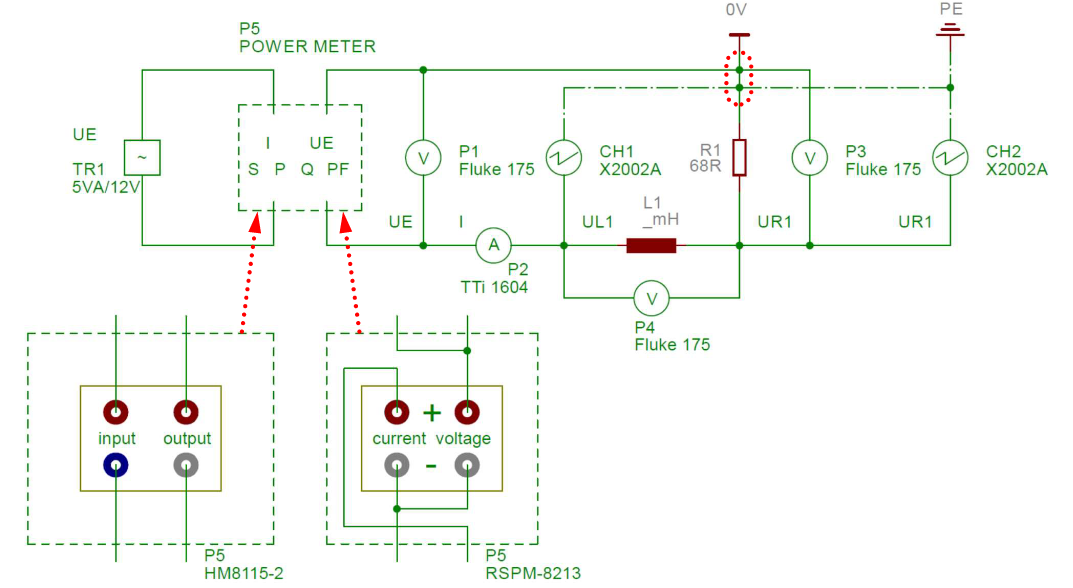
\includegraphics[scale=1]{bilder/aufbau_task5.png}
\end{figure}




\section{Versuchsdurchführung und Messwerte}

\subsection{Untersuchung  der  Anzeige  von  unterschiedlichen  Spannungsmessinstrumenten  bei verschiedenen Kurvenformen}

Abschnitt~\ref{subsec:aufbau_task1} beschreibt den Aufbau des Versuchs. Dieser wird nun mit einer Sinusspannung, einer Dreiecksspannung und einer Rechtecksspannung durchgeführt. Das Oszilloskop zeichnet diese 3 Kurven. Sie sind in Grafiken \ref{fig:task1_sin}, \ref{fig:task1_dreieck} und \ref{fig:task1_rechteck} dargestellt.


\begin{figure}[H]
\centering
\caption{Sinusschwingung für Aufgabe 1}
\label{fig:task1_sin}
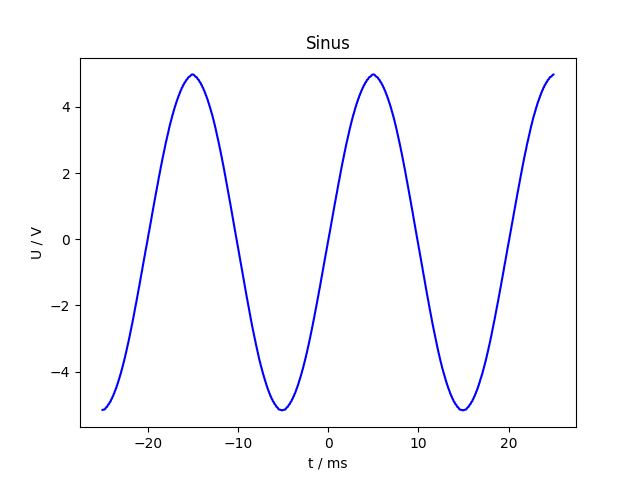
\includegraphics[scale=0.5]{bilder/task1_sin.png}
\end{figure}

\begin{figure}[H]
\centering
\caption{Dreiecksschwingung für Aufgabe 1}
\label{fig:task1_dreieck}
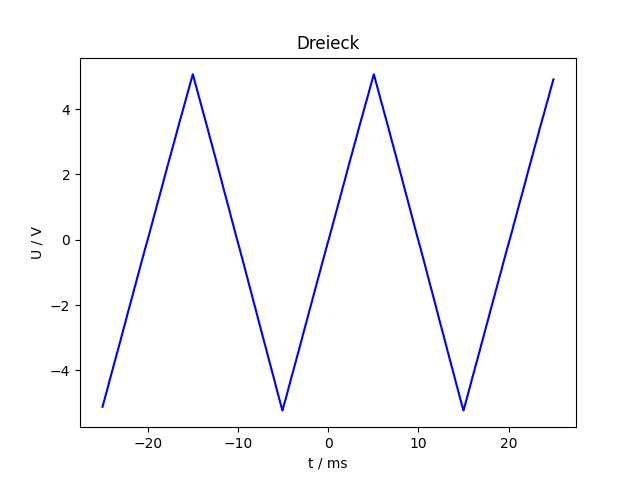
\includegraphics[scale=0.5]{bilder/task1_dreieck.png}
\end{figure}

\begin{figure}[H]
\centering
\caption{Rechtecksschwingung für Aufgabe 1}
\label{fig:task1_rechteck}
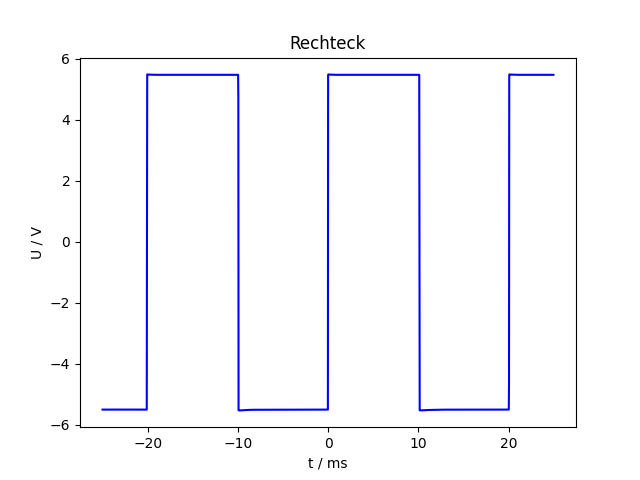
\includegraphics[scale=0.5]{bilder/task1_rechteck.png}
\end{figure}


Die gemessenen Werte werden in Tabellen~\ref{tab:messung_task1_volt} und~\ref{tab:messung_task1_oszi} zusammengefasst.

\begin{table}[H]
\centering
\caption{Gemessene Effektivwerte im Versuch 1 mit 3 verschiedenen Messgeräten. $U_1$ ist TTi1604, $U_2$ ist M4600 und $U_3$ ist Unigor 4.}
\label{tab:messung_task1_volt}
\begin{tabular}{r|rrr}
Schwingung & $U_{1,\text{eff}}$ / V  & $U_{2,\text{eff}}$ / V & $U_{3,\text{eff}}$ / V \\
\hline
Sinus & 3.532 & 3.535 & 3.31 \\
Dreieck & 2.965 & 2.863 & 2.66 \\
Rechteck & 5.500 & 6.003 & 5.91
\end{tabular}
\end{table}


\begin{table}[H]
\centering
\caption{Messwerte bei Versuch 1 mit Oszilloskop.}
\label{tab:messung_task1_oszi}
\begin{tabular}{r|rr}
Schwingung &  $U_{ss}$ / V &  $U_\text{eff}$ / V  \\
\hline
Sinus & 10.15 & 3.55 \\
Dreieck & 10.28 & 2.97 \\
Rechteck & 11.01 & 5.48
\end{tabular}
\end{table}



\subsection{Phasenlage von Strom und Spannung an einem Kondensator bzw. einer Spule}

In diesem Fall werden beide Versuchsaufbauten (Grafiken~\ref{fig:aufbau_task2} und \ref{fig:aufbau_task3}) vermessen und man erhält die jeweiligen Kurven. Diese sind in Grafiken~\ref{fig:task2_kurve} und \ref{fig:task3_kurve} zu sehen. Gemäß der jeweiligen Versuchsaufbauten ist CH1 proportional zu den Strom durch Spule bzw. Kondensator. Man erkennt in Grafik~\ref{fig:task2_kurve} deutlich, dass der Strom (CH1) der Spannung (CH2) vorausgeht. Bei der Spule in Grafik~\ref{fig:task3_kurve} ist es genau umgekehrt.

\begin{figure}[H]
\centering
\caption{Kurve des Kondensators aus Aufgabe 2}
\label{fig:task2_kurve}
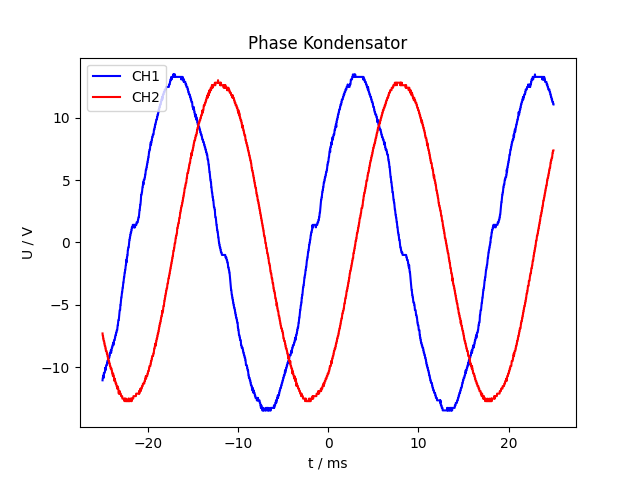
\includegraphics[scale=0.5]{bilder/task2.png}
\end{figure}

\begin{figure}[H]
\centering
\caption{Kurve der Spule aus Aufgabe 3}
\label{fig:task3_kurve}
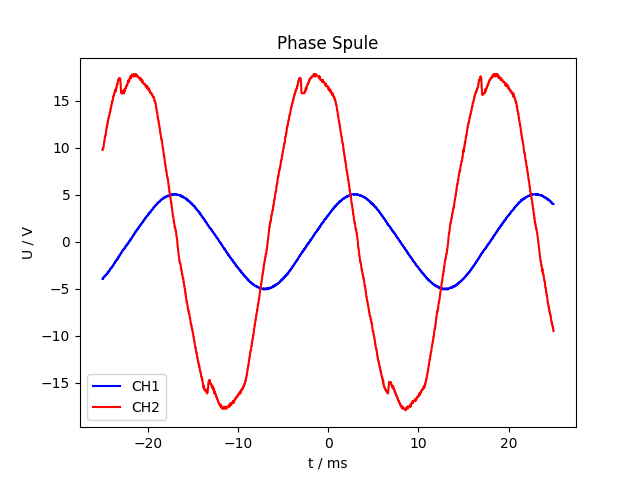
\includegraphics[scale=0.5]{bilder/task3.png}
\end{figure}







\section{Auswertung}

\subsection{Untersuchung  der  Anzeige  von  unterschiedlichen  Spannungsmessinstrumenten  bei verschiedenen Kurvenformen }

Aus der Kurve soll nun der Spitze-Tal-Wert und der Effektivwert berechnet werden. Hierfür wird die Periodendauer benötigt, die sich aus der Frequenz von $f=50~$Hz ergibt. Diese wäre $\tau = 50.00~$ms.

Die Spitze-Tal Werte wurden berechnet, indem zuerst das globale Minimum bzw das globale Maximum der gesamten gegeben Kurve berechnet wurden und diese anschließend voneinander subtrahiert wurden. Der Algorithmus ist in Listing~\ref{lst:ss} beschrieben.

\lstinputlisting[language=Python,captionpos=b, label=lst:ss,caption={Python Skript zur Bestimmung des Spitze-Tal Wertes}]{scripts/spitze_tal.py}



Zusätzlich wurde für die Effektivwerte eine numerische Integration durchgeführt. Hierfür wurde auf die Simpson-Formel zurückgegriffen. Diese findet sich im Python-Paket \texttt{scipy}. Im Falle der Sinus-Schwingung und der Dreiecksschwingung wurde über die eine Periode von 2 benachbarten Maxima integriert. Bei der Rechtecksschwigung wurde zwischen 2 steigenden Flanken des Rechtecks integriert. 





Daraus ergeben sich die Werte in Tabelle~\ref{tab:task1_ergebnisse}.
\begin{table}[H]
\caption{Spitze-Tal Werte für die Kurven.}
\label{tab:task1_ergebnisse}
\begin{tabular}{c|cc}
Schwingung & $U_\text{ss}$ / V & $U_\text{eff}$ / V  \\
\hline
Sinus & 10.15 & 3.56 \\
Dreieck & 10.29 & 2.98 \\
Rechteck & 11.01 & 5.49
\end{tabular}
\end{table}



\subsection{Phasenlage von Strom und Spannung an einem Kondensator bzw. einer Spule}

Die Phasenverschiebung kann theoretisch und praktisch berechnet werden. Gemäß der Formel für die Impedanz ergibt sich nach der Theorie (vgl. \cite{demtroeder})
\begin{align*}
Z_2 &= R + Z_{C_1} = R - \frac{i}{2\cdot\pi\cdot f \cdot C_1} \\
Z_3 &= R + Z_{L} = R + i\cdot 2\cdot\pi\cdot f \cdot L
\end{align*}
für die Gesamtimpedanz in den Versuchen 2 und 3.

Für die Phasenverschiebung beim Kondensator aus Aufgabe 2 ($\varphi_2$) gilt daher
\begin{align*}
\tan\left(\varphi_2\right) &= \frac{\Im(Z_2)}{\Re(Z_2)} \\
&= \frac{1}{2\cdot\pi} \cdot\left(\frac{1}{ f\cdot R \cdot C_1} \pm  \frac{\Delta f\cdot R \cdot C_1 + f\cdot \Delta R \cdot C_1 + f\cdot R \cdot \Delta C_1}{ (f \cdot R\cdot C_1)^2} \right)
\end{align*}

Für die Phasenverschiebung bei der Spule aus Aufgabe 3 ($\varphi_3$) gilt nach der Theorie
\begin{align*}
\tan\left(\varphi_3\right) &= \frac{\Im(Z_3)}{\Re(Z_3)} \\
&= 2\cdot \pi\cdot \left( \frac{f \cdot L}{R} \pm \frac{\Delta f\cdot L\cdot R + f\cdot \Delta L\cdot R + f\cdot L \cdot \Delta R}{R^2} \right)
\end{align*}


Für Aufgabe 2 ergibt sich ein theoretischer Wert $\varphi_2 = (44 \pm 8)^\circ$, die sich der Strom vor der Spannung eines Kondensators befindet. Da für die Spule keine Induktion gegeben ist, kann der theoretische Wert nicht berechnet werden.



\section{Diskussion}


\subsection{Untersuchung  der  Anzeige  von  unterschiedlichen  Spannungsmessinstrumenten  bei verschiedenen Kurvenformen }

Tabelle~\ref{tab:task1_final} zeigt alle berechneten Ergebnisse der Effektivwerte. Generell ist zu sagen, dass die meisten Messgeräte für Sinus-Schwingungen ausgelegt sind und alle anderen Schwingungen durch Sinus-Schwingungen approximieren. Dadurch muss man diese händisch umrechnen. Alternativ kann man die Kurve numerisch integrieren, um auf eine genauere Berechnung zu kommen. Dies ist insbesondere vorteilhaft, falls es bei der Sinus-Schwingung selbst zu möglichen Unregelmäßigkeiten oder Verzerrungen kommt. Das Oszilloskop selbst benutzt zur Berechnung des Effektivwertes auch eine numerische Integration. Dieser Schluss ergibt sich, wenn man die Zahlen vergleicht. Die Messgeräte TTi1604 und M4600 erhalten bei der Sinusschwingung durchaus akzeptable Werte. Lediglich Unigor 4 weicht bei der Sinusschwingung um 0.2~V ab.

Es sollte zusätzlich noch kritisch hinterfragt werden, ob sich die Messgeräte bei gleichzeitiger Messung gegenseitig beeinflussen.

Im Allgemeinen zeigt sich (wie es sich auch geometrisch vermuten lässt), dass bei nicht exakter Berechnung die Dreiecksspannung einen kleineren Wert ergibt, und die Rechtecksspannung einen größeren. Das liegt an der geometrischen Überlegung, dass die Fläche unter der Dreiecksschwingung kleiner ist als jene bei einer Sinusschwingung und jene eines Rechtecks größer.

\subsection{Phasenlage von Strom und Spannung an einem Kondensator bzw. einer Spule}

Für den Kondensator wurde eine Phasenverschiebung von $\varphi_2 = 92.30^\circ$ gemessen. Das ist nach der Theorie nicht möglich, da ein perfekter Kondensator ohne Widerstand eine Impedanz von 
\begin{align*}
Z_C = \frac{1}{i\cdot\omega \cdot C}
\end{align*}
aufweist. In der Beziehung $U=Z_C\cdot I$ entsteht dadurch eine $90^\circ$ Phasenverschiebung zwischen $I$ und $U$. Der Isolationswiderstand, welcher in \cite{moodle} beschrieben ist, würde diese Phasenverschiebung höchstens verkleinern. Der theoretische Wert der Phasenverschiebung wäre $\varphi_2 = (44\pm8)^\circ$ unter Vernachlässigung des Isolationswiderstandes und der Annahme eines perfekten Kondensators für die gegebenen Werte $R = 68~\Omega$, $f=50~$Hz und $C=47~\mu$F.

~

Die Impedanz einer Spule wäre 
\begin{align*}
Z_L = i\cdot\omega \cdot L
\end{align*}
Analog könnte man bei gegebener Induktivität einen theoretischen Wert für die Phasenverschiebung berechnen, sofern $L$ gegeben wäre. Die Phasenverschiebung würde sich durch das Vorzeichen von jener beim Kondensator unterscheiden.


\subsection{Leistung einer RC- bzw RL-Schaltung}




\section{Zusammenfassung}

\subsection{Untersuchung  der  Anzeige  von  unterschiedlichen  Spannungsmessinstrumenten  bei verschiedenen Kurvenformen }


\begin{table}[H]
\centering
\caption{Gemessene Effektivwerte mit 3 verschiedenen Messgeräten und dem Oszilloskop. $U_1$ ist TTi1604, $U_2$ ist M4600 und $U_3$ ist Unigor 4.}
\label{tab:task1_final}
\begin{tabular}{r|rrrr|p{2cm}}
Schwingung & Oszi\-loskop & $U_{1,\text{eff}}$ / V  & $U_{2,\text{eff}}$ / V & $U_{3,\text{eff}}$ / V & berechneter Effektivwert\\
\hline
Sinus & 3.55 & 3.532 & 3.535 & 3.31 & \hfill3.56\\
Dreieck & 2.97 & 2.965 & 2.863 & 2.66 & \hfill2.98 \\
Rechteck & 5.48 & 5.500 & 6.003 & 5.91 & \hfill5.49
\end{tabular}
\end{table}



\subsection{Phasenlage von Strom und Spannung an einem Kondensator bzw. einer Spule}


\subsection{Leistung einer RC- bzw RL-Schaltung}




\begin{thebibliography}{9}
\bibitem{moodle} Moodle-Unterlagen zum Versuch, bereitgestellt von der Karl-Franzens-Universität Graz.
\bibitem{src2} \url{https://www.spektrum.de/lexikon/physik/wechselstrom/15456}
\bibitem{src3} \url{https://www.leifiphysik.de/elektrizitaetslehre/wechselstromtechnik/grundwissen/effektivwerte-von-wechselstrom-und-spannung}
\bibitem{src4} \url{https://www.lernhelfer.de/schuelerlexikon/physik-abitur/artikel/wechselspannung-und-wechselstrom}
\bibitem{src5} \url{https://www.chemie-schule.de/KnowHow/Gleichrichtwert}
\bibitem{src6} \url{https://www.emf.ethz.ch/emf-info/themen/physik/verknuepfung-von-elektrischen-und-magnetischen-feldern/wirkleistung-blindleistung-scheinleistung/}

\bibitem{demtroeder} W. Demtröder: \emph{Experimentalphysik 2 - Elektrizität  und Optik}, 7. Auflage, 2017.
\end{thebibliography}


%\newpage 
%\appendix
%\section{Python Skript}



%\lstinputlisting[language=Python,captionpos=b, label=lst:test,caption={Python Skript}]{plot.py}

%\lstinputlisting[language=Python,captionpos=b, label=lst:test,caption={Bessel Auswertung}]{generate_numbers_bessel.py}


%\lstinputlisting[language=Python,captionpos=b, label=lst:test,caption={Zerstreuungslinse Auswertung}]{generate_numbers_zerstreuungslinse.py}


\end{document}
